\documentclass{article}

\usepackage[a4paper, left=1.5cm, right=1.5cm, top=2cm, bottom=2cm]{geometry}

\usepackage{../../../components/components} % <-- ton fichier .sty, avec toutes tes définitions

\usepackage{fancyhdr}


% Configuration des en-têtes et pieds de page
\pagestyle{fancy}
\fancyhf{} % reset tout

\fancyhead[L]{DL Math-Info}
\fancyhead[C]{Fichier de tests}
\fancyhead[R]{2025-2026}

\fancyfoot[L]{Ewen Rodrigues de Oliveira}
\fancyfoot[R]{\thepage}

\begin{document}

\docTitle{Chapitre 0 : Tests}

\section{Matrices}

\example{Incididunt voluptate est magna reprehenderit excepteur commodo cupidatat labore laborum et enim. $\begin{pmatrix}
    a & b & c \\
    d & 0 & 2 
\end{pmatrix}$ après.}


\begin{lstlisting}[language=Python]
def seuil(n):
    for i in range(len(n)):
        if n[i] < 0:
            return i
    return len(n)
\end{lstlisting}

\theorem{Proposition}{Graphe de la fonction tangeante}{true}{
    Soit \( tan : \mathbb{R} \to \mathbb{R} \) la fonction tangente. Alors son graphe est défini par :
    \[
    \Gamma_{tan} = \{ (x, tan(x)) \in \mathbb{R}^2 \mid x \in \mathbb{R} \}
    \]

    On a le graphique suivant : 
    \begin{center}
        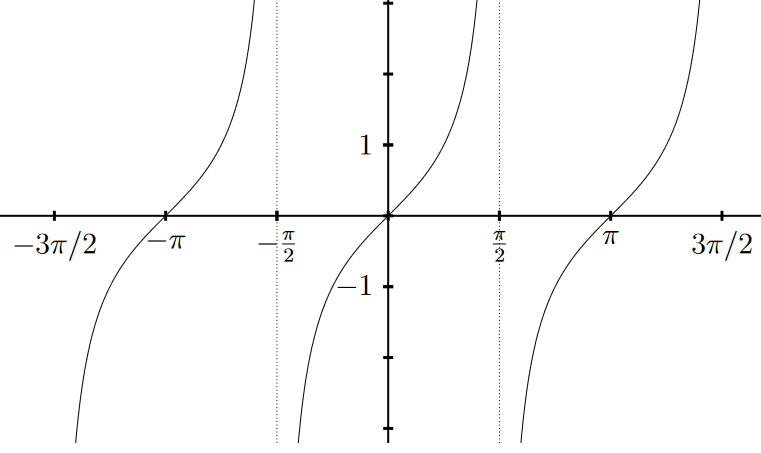
\includegraphics[width=0.5\textwidth]{./images/tan.png}
        \captionof{figure}{Graphe de la fonction tangente sur \([- \pi/2, \pi/2]\).}
    \end{center}

}

\training{Test sur $2^n$ ou $2_n$ ou $2^n_i$}

\end{document}